\documentclass[aspectratio=169]{beamer}
\usepackage{lmodern}
%\usetheme{Madrid}
%\usecolortheme{giantoak}
\newcommand*\oldmacro{}
\let\oldmacro\insertshorttitle
\renewcommand*\insertshorttitle{\oldmacro\hfill\insertframenumber\,/\,\inserttotalframenumber}
\usepackage[framemethod=tikz]{mdframed}

%\usepackage{beamerthemesplit}
\usepackage{textpos}
\usepackage{pgf}
\usepackage{ulem}
%\logo{\pgfputat{\pgfxy(0,-.4)}{\pgfbox[right,base]{\includegraphics[height=1.0cm]{logo.jpg}}}}
%\newcommand{\nologo}{\setbeamertemplate{logo}{}}
\usepackage{booktabs}
\usepackage{graphicx}
\theoremstyle{principle}
\newtheorem*{principle}{Design Principle}


\titlegraphic{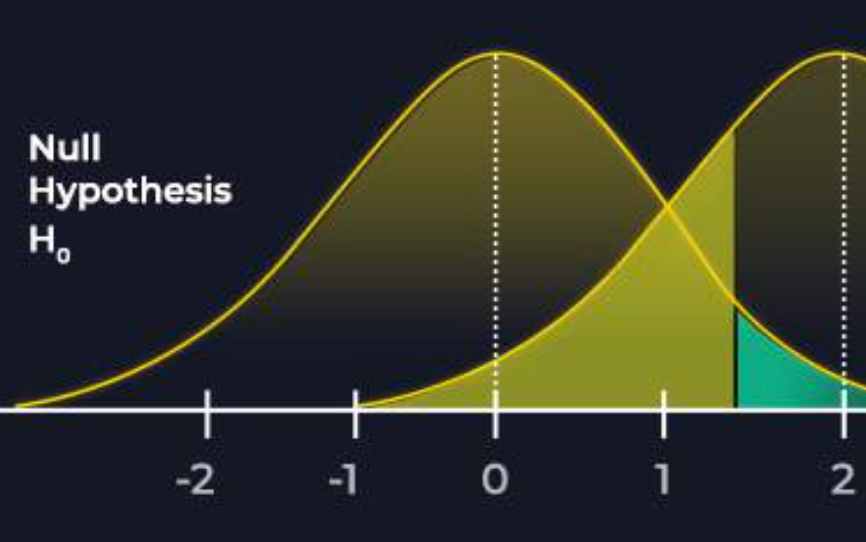
\includegraphics[width=1.0\paperwidth]{distros.png}}

\title{Amendments}
%\author[Jeremy Kedziora]{Wind Data Science Team\\
%\small{Uptake}}
\date{}

\begin{document}

%{
%%\nologo
%\begin{frame}
%    \maketitle
%\end{frame}
%}
%pages 1-7, 8-9, 14-15.


{
%  \usebackgroundtemplate{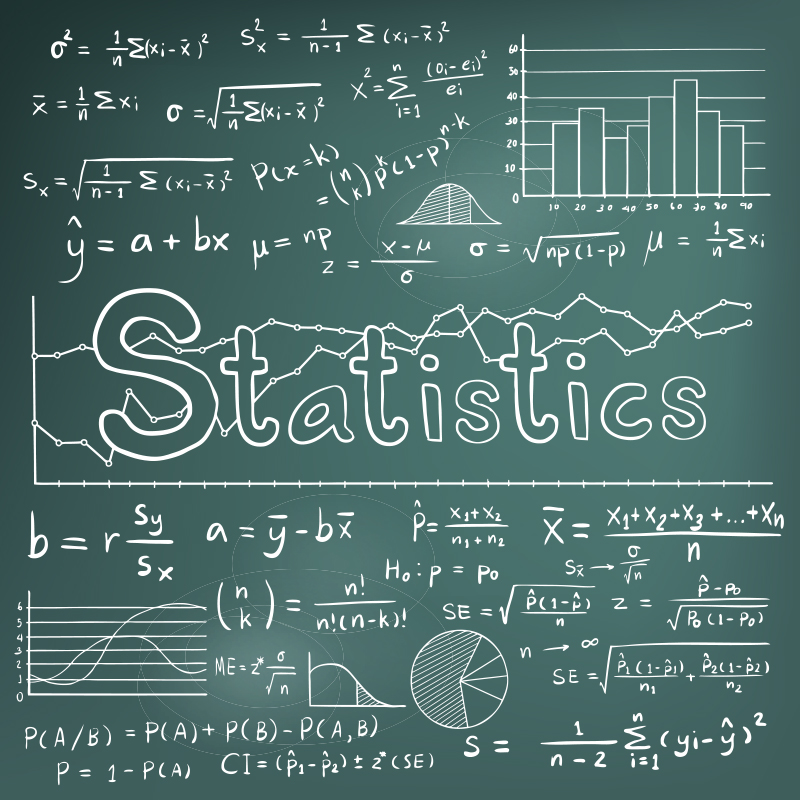
\includegraphics[width=1.0\paperwidth]{statistics-review.jpg}}
  \usebackgroundtemplate{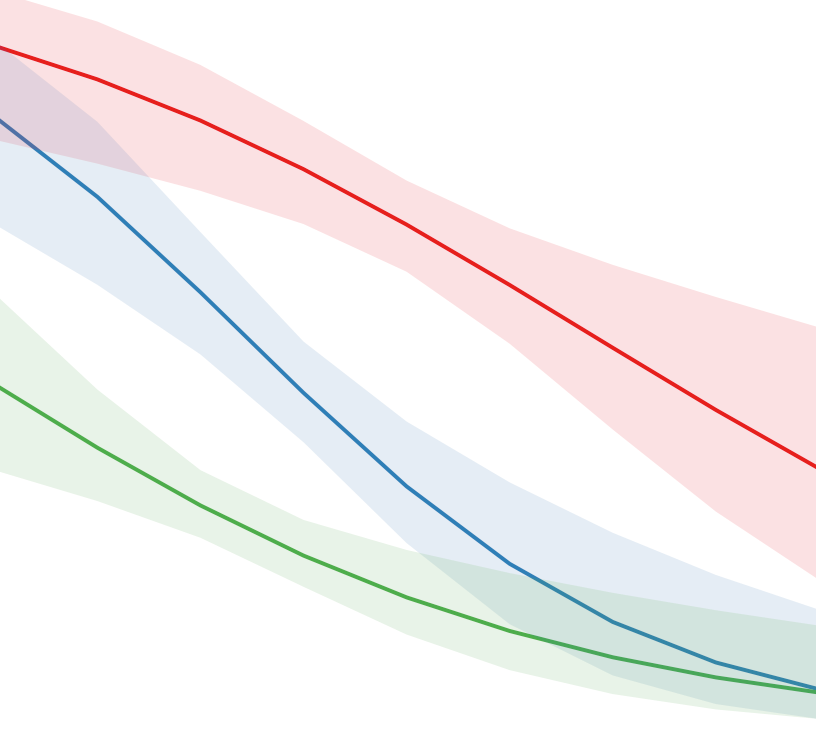
\includegraphics[scale=1.1]{interaction_terms.png}}
  \begin{frame}[plain]
  
\begin{mdframed}[tikzsetting={draw=white,fill=white,fill opacity=0.6,draw opacity=0.4,
               line width=0pt},backgroundcolor=none,leftmargin=20,
               rightmargin=20,innertopmargin=4pt]
\begin{center}
\Huge \textbf{Variable Interactions}
\end{center}
\end{mdframed}

  \end{frame}
}

%most reliant on human cognition
%limited only by cognition
%hypothesis generating scheme often functioning as a gateway into more statistical analysis

%%@@@@@@@@@@@@@@@@@@@@@@@@@@@@@@@@@@@@@@@@@@@@@@@@@
%\begin{frame}
%\frametitle{Napoleon's Progress}
%\begin{center}
%
\includegraphics[scale=0.4]{experiment.png}
%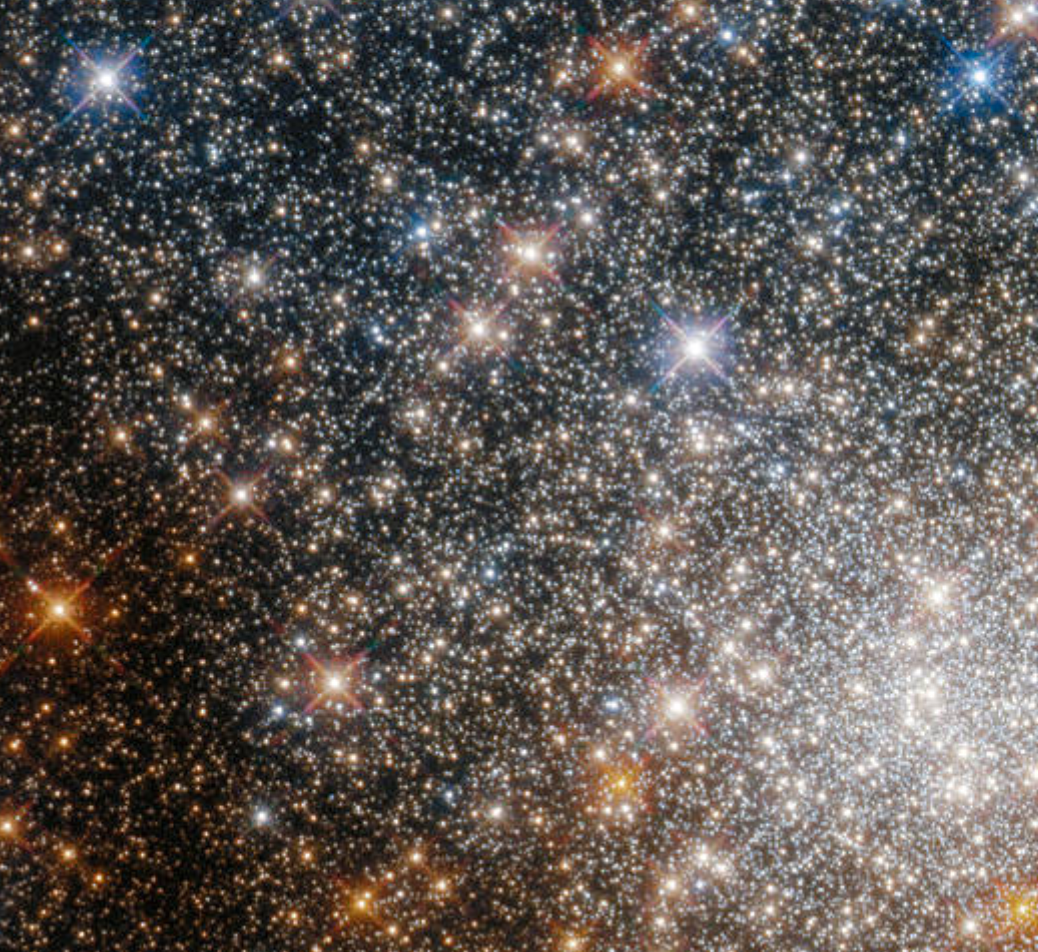
\includegraphics[scale=0.35]{stars.png}
%\end{center}
%
%\end{frame}

%@@@@@@@@@@@@@@@@@@@@@@@@@@@@@@@@@@@@@@@@@@@@@@@@@
\begin{frame}
\frametitle{Today:}

\begin{itemize}
\item Define variable interactions in a linear regression context.
\bigskip
\bigskip
\bigskip

\item Understand how to interpret the coefficients and $p$-values for variable interactions.

\end{itemize}

\end{frame}

%@@@@@@@@@@@@@@@@@@@@@@@@@@@@@@@@@@@@@@@@@@@@@@@@@
\begin{frame}
\frametitle{What are \textbf{variable interactions}?}

\begin{itemize}
\item So far, we've used linear regression to:
\begin{enumerate} 
\item Model a linear relationship between dependent variable $y$ and independent variable $x$:
\begin{align*}
y = \beta_0 + \beta_1x + \varepsilon;
\end{align*}
\item Model a linear relationship between dependent variable $y$ and many independent variables $x_1,x_2,x_3,\hdots$:
\begin{align*}
y = \beta_0 + \beta_1x_1 + \beta_2x_2 + \beta_3x_3 + \hdots + \varepsilon;
\end{align*}
\item Model a NON-linear relationship between dependent variable $y$ and many independent variables $x$:
\begin{align*}
y = \beta_0 + \beta_1x_1 + \beta_2x_1^2 + \hdots + \varepsilon;
\end{align*}
\end{enumerate}

\item[]\color{white} But what if the effect of one independent variable depends on another independent variable?!

\end{itemize}

\end{frame}

%@@@@@@@@@@@@@@@@@@@@@@@@@@@@@@@@@@@@@@@@@@@@@@@@@
\begin{frame}
\frametitle{What are \textbf{variable interactions}?}

\begin{itemize}
\item So far, we've used linear regression to:
\begin{enumerate} 
\item Model a linear relationship between dependent variable $y$ and independent variable $x$:
\begin{align*}
y = \beta_0 + \beta_1x + \varepsilon;
\end{align*}
\item Model a linear relationship between dependent variable $y$ and many independent variables $x_1,x_2,x_3,\hdots$:
\begin{align*}
y = \beta_0 + \beta_1x_1 + \beta_2x_2 + \beta_3x_3 + \hdots + \varepsilon;
\end{align*}
\item Model a NON-linear relationship between dependent variable $y$ and many independent variables $x$:
\begin{align*}
y = \beta_0 + \beta_1x_1 + \beta_2x_1^2 + \hdots + \varepsilon;
\end{align*}
\end{enumerate}

\item But what if the effect of one independent variable depends on another independent variable?!

\end{itemize}

\end{frame}

%@@@@@@@@@@@@@@@@@@@@@@@@@@@@@@@@@@@@@@@@@@@@@@@@@
\begin{frame}
\frametitle{What are \textbf{variable interactions}?}

\begin{center}
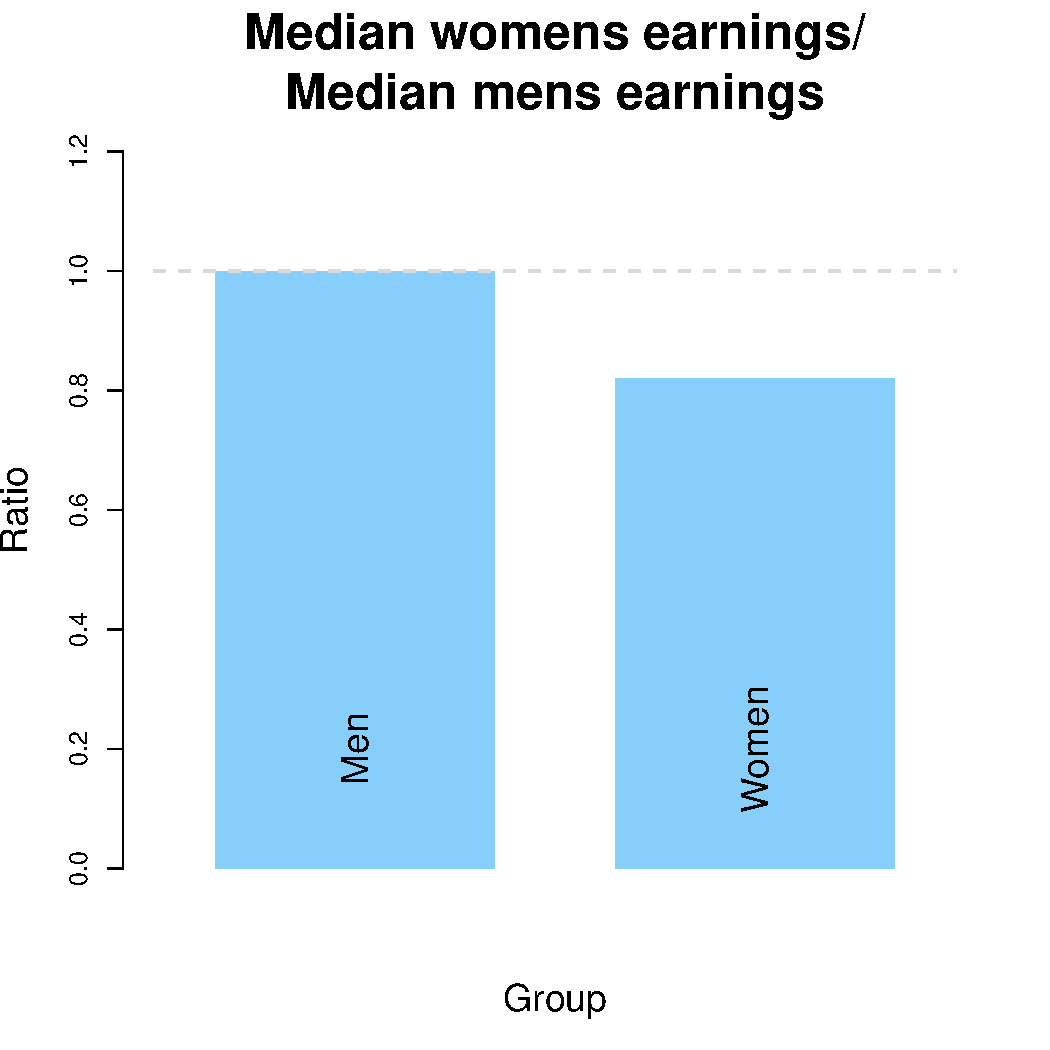
\includegraphics[scale=0.4]{gender_wage_gap.pdf}
\end{center}

\end{frame}

%@@@@@@@@@@@@@@@@@@@@@@@@@@@@@@@@@@@@@@@@@@@@@@@@@
\begin{frame}
\frametitle{What are \textbf{variable interactions}?}

\begin{center}
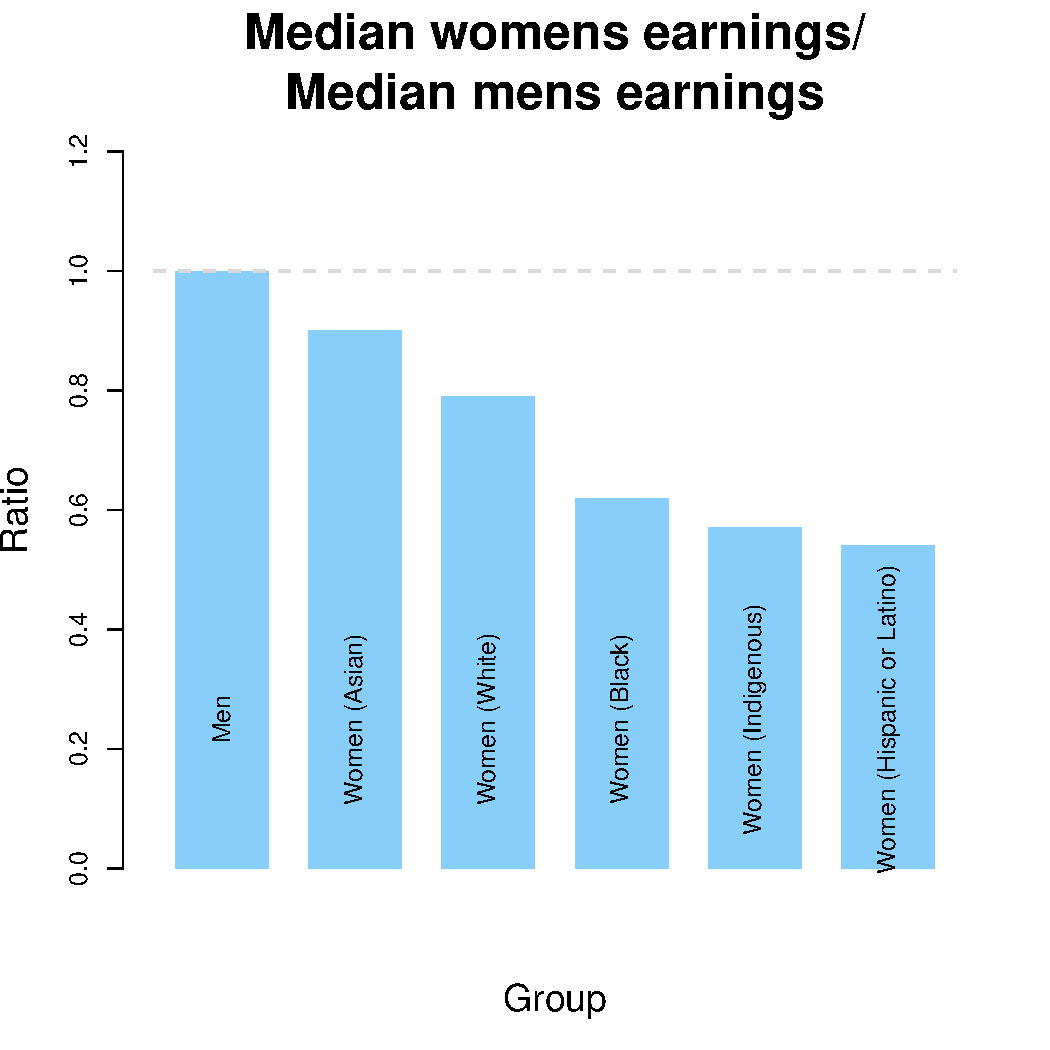
\includegraphics[scale=0.4]{gender_wage_gap_DA.pdf}
\end{center}

\end{frame}

%%@@@@@@@@@@@@@@@@@@@@@@@@@@@@@@@@@@@@@@@@@@@@@@@@@
%\begin{frame}
%\frametitle{What does nonlinearity look like?}
%
%\begin{columns}
%\begin{column}{0.4\textwidth}
%
%\begin{itemize}
%\item Linear regression allows us to model a linear relationship between $x$ and $y$;
%\bigskip
%\bigskip
%\bigskip
%
%\item[]\color{white} But what if the data looks like this?!
%
%\end{itemize}
%
%\end{column}
%\begin{column}{0.6\textwidth}
%\begin{center}
%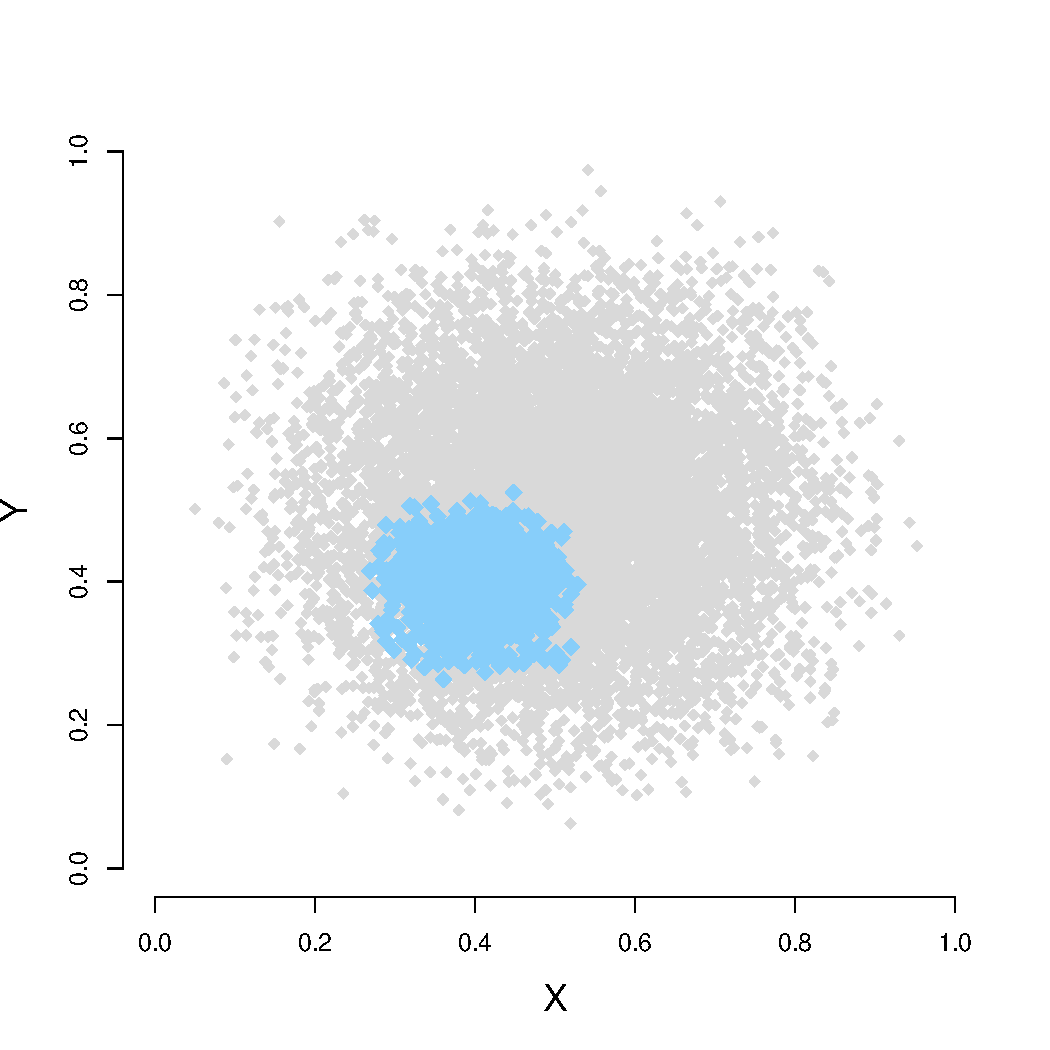
\includegraphics[scale=0.45]{point_cloud.pdf}
%\end{center}
%\end{column}
%\end{columns}
%
%\end{frame}

%@@@@@@@@@@@@@@@@@@@@@@@@@@@@@@@@@@@@@@@@@@@@@@@@@
\begin{frame}
\frametitle{What are \textbf{variable interactions}?}


\huge
\begin{align*}
y = \beta_0 + \beta_1x_1 + \beta_2x_2 + \hdots + \varepsilon
\end{align*}
\bigskip
\normalsize
\begin{itemize}
\item $y$ is the \textbf{dependent variable} -- this is part of the data set;
\item The $x$'s are \textbf{independent variables} that explain $y$ -- also part of the data set;
\item The $\beta$'s are called \textbf{coefficient effects} that control how the $x$'s affect $y$ -- they are \textbf{learned} from the data;
\item The $\varepsilon$ is a \textbf{noise} term.

\end{itemize}
\bigskip
\bigskip


\end{frame}

%@@@@@@@@@@@@@@@@@@@@@@@@@@@@@@@@@@@@@@@@@@@@@@@@@
\begin{frame}
\frametitle{What are \textbf{variable interactions}?}


\huge
\begin{align*}
y = \beta_0 + \beta_1x_1 + \beta_2x_2 + \underbrace{\beta_{12}x_1x_2}_{\mbox{\normalsize interaction}} + \hdots + \varepsilon
\end{align*}
\bigskip
\normalsize
\begin{itemize}
\item $y$ is the \textbf{dependent variable} -- this is part of the data set;
\item The $x$'s are \textbf{independent variables} that explain $y$ -- also part of the data set;
\item The $\beta$'s are called \textbf{coefficient effects} that control how the $x$'s affect $y$ -- they are \textbf{learned} from the data;
\item The $\varepsilon$ is a \textbf{noise} term.

\end{itemize}
\bigskip
\bigskip


\end{frame}

%@@@@@@@@@@@@@@@@@@@@@@@@@@@@@@@@@@@@@@@@@@@@@@@@@
\begin{frame}
\frametitle{Interpreting variable interactions: coefficients}

What is the effect of a unit increase in $x_1$ on y?
\begin{align*}
y_1 &= \beta_0 + \beta_1x_1 + \beta_2x_2 + \beta_{12}x_1x_2\\
\color{white}\mbox{for a unit increase in $x_1$: } y_2 &\color{white}= \beta_0 + \beta_1(x_1 + 1) + \beta_2x_2 + \beta_{12}(x_1 + 1)x_2\\
\color{white}&\color{white}= \beta_0 + \beta_1x_1 + \beta_1 + \beta_2x_2 + \beta_{12}x_1x_2 + \beta_{12}x_2\\
\color{white}\mbox{so change in $y$ is: }y_2 - y_1 &\color{white}= \underbrace{\beta_0 + \beta_1x_1 + \beta_1 + \beta_2x_2 + \beta_{12}x_1x_2 + \beta_{12}x_2}_{y_2}\\
\color{white}&\color{white}\hspace{25mm} - (\underbrace{\beta_0 + \beta_1x_1 + \beta_2x_2 + \beta_{12}x_1x_2}_{y_1})\\
\color{white}&\color{white}= \beta + \beta_{12}x_2.
\end{align*}

\end{frame}


%@@@@@@@@@@@@@@@@@@@@@@@@@@@@@@@@@@@@@@@@@@@@@@@@@
\begin{frame}
\frametitle{Interpreting variable interactions: coefficients}

What is the effect of a unit increase in $x_1$ on y?
\begin{align*}
y_1 &= \beta_0 + \beta_1x_1 + \beta_2x_2 + \beta_{12}x_1x_2\\
\mbox{for a unit increase in $x_1$: } y_2 &= \beta_0 + \beta_1(x_1 + 1) + \beta_2x_2 + \beta_{12}(x_1 + 1)x_2\\
\color{white}&\color{white}= \beta_0 + \beta_1x_1 + \beta_1 + \beta_2x_2 + \beta_{12}x_1x_2 + \beta_{12}x_2\\
\color{white}\mbox{so change in $y$ is: }y_2 - y_1 &\color{white}= \underbrace{\beta_0 + \beta_1x_1 + \beta_1 + \beta_2x_2 + \beta_{12}x_1x_2 + \beta_{12}x_2}_{y_2}\\
\color{white}&\color{white}\hspace{25mm} - (\underbrace{\beta_0 + \beta_1x_1 + \beta_2x_2 + \beta_{12}x_1x_2}_{y_1})\\
\color{white}&\color{white}= \beta + \beta_{12}x_2.
\end{align*}

\end{frame}

%@@@@@@@@@@@@@@@@@@@@@@@@@@@@@@@@@@@@@@@@@@@@@@@@@
\begin{frame}
\frametitle{Interpreting variable interactions: coefficients}

What is the effect of a unit increase in $x_1$ on y?
\begin{align*}
y_1 &= \beta_0 + \beta_1x_1 + \beta_2x_2 + \beta_{12}x_1x_2\\
\mbox{for a unit increase in $x_1$: } y_2 &= \beta_0 + \beta_1(x_1 + 1) + \beta_2x_2 + \beta_{12}(x_1 + 1)x_2\\
&= \beta_0 + \beta_1x_1 + \beta_1 + \beta_2x_2 + \beta_{12}x_1x_2 + \beta_{12}x_2\\
\color{white}\mbox{so change in $y$ is: }y_2 - y_1 &\color{white}= \underbrace{\beta_0 + \beta_1x_1 + \beta_1 + \beta_2x_2 + \beta_{12}x_1x_2 + \beta_{12}x_2}_{y_2}\\
\color{white}&\color{white}\hspace{25mm} - (\underbrace{\beta_0 + \beta_1x_1 + \beta_2x_2 + \beta_{12}x_1x_2}_{y_1})\\
\color{white}&\color{white}= \beta + \beta_{12}x_2.
\end{align*}

\end{frame}

%@@@@@@@@@@@@@@@@@@@@@@@@@@@@@@@@@@@@@@@@@@@@@@@@@
\begin{frame}
\frametitle{Interpreting variable interactions: coefficients}

What is the effect of a unit increase in $x_1$ on y?
\begin{align*}
y_1 &= \beta_0 + \beta_1x_1 + \beta_2x_2 + \beta_{12}x_1x_2\\
\mbox{for a unit increase in $x_1$: } y_2 &= \beta_0 + \beta_1(x_1 + 1) + \beta_2x_2 + \beta_{12}(x_1 + 1)x_2\\
&= \beta_0 + \beta_1x_1 + \beta_1 + \beta_2x_2 + \beta_{12}x_1x_2 + \beta_{12}x_2\\
\mbox{so change in $y$ is: }y_2 - y_1 &= \color{white}\underbrace{\beta_0 + \beta_1x_1 + \beta_1 + \beta_2x_2 + \beta_{12}x_1x_2 + \beta_{12}x_2}_{y_2}\\
\color{white}&\color{white}\hspace{25mm} - (\underbrace{\beta_0 + \beta_1x_1 + \beta_2x_2 + \beta_{12}x_1x_2}_{y_1})\\
\color{white}&\color{white}= \beta + \beta_{12}x_2.
\end{align*}

\end{frame}

%@@@@@@@@@@@@@@@@@@@@@@@@@@@@@@@@@@@@@@@@@@@@@@@@@
\begin{frame}
\frametitle{Interpreting variable interactions: coefficients}

What is the effect of a unit increase in $x_1$ on y?
\begin{align*}
y_1 &= \beta_0 + \beta_1x_1 + \beta_2x_2 + \beta_{12}x_1x_2\\
\mbox{for a unit increase in $x_1$: } y_2 &= \beta_0 + \beta_1(x_1 + 1) + \beta_2x_2 + \beta_{12}(x_1 + 1)x_2\\
&= \beta_0 + \beta_1x_1 + \beta_1 + \beta_2x_2 + \beta_{12}x_1x_2 + \beta_{12}x_2\\
\mbox{so change in $y$ is: }y_2 - y_1 &= \underbrace{\beta_0 + \beta_1x_1 + \beta_1 + \beta_2x_2 + \beta_{12}x_1x_2 + \beta_{12}x_2}_{y_2}\\
&\hspace{25mm} - (\underbrace{\beta_0 + \beta_1x_1 + \beta_2x_2 + \beta_{12}x_1x_2}_{y_1})\\
\color{white}&\color{white}= \beta + \beta_{12}x_2.
\end{align*}

\end{frame}

%@@@@@@@@@@@@@@@@@@@@@@@@@@@@@@@@@@@@@@@@@@@@@@@@@
\begin{frame}
\frametitle{Interpreting variable interactions: coefficients}

What is the effect of a unit increase in $x_1$ on y?
\begin{align*}
y_1 &= \beta_0 + \beta_1x_1 + \beta_2x_2 + \beta_{12}x_1x_2\\
\mbox{for a unit increase in $x_1$: } y_2 &= \beta_0 + \beta_1(x_1 + 1) + \beta_2x_2 + \beta_{12}(x_1 + 1)x_2\\
&= \beta_0 + \beta_1x_1 + \beta_1 + \beta_2x_2 + \beta_{12}x_1x_2 + \beta_{12}x_2\\
\mbox{so change in $y$ is: }y_2 - y_1 &= \underbrace{\beta_0 + \beta_1x_1 + \beta_1 + \beta_2x_2 + \beta_{12}x_1x_2 + \beta_{12}x_2}_{y_2}\\
&\hspace{25mm} - \underbrace{\beta_0 - \beta_1x_1 - \beta_2x_2 - \beta_{12}x_1x_2}_{y_1}\\
&= \beta_1 + \beta_{12}x_2.
\end{align*}

\end{frame}

%@@@@@@@@@@@@@@@@@@@@@@@@@@@@@@@@@@@@@@@@@@@@@@@@@
\begin{frame}
\frametitle{What does this actually look like?}

\begin{center}
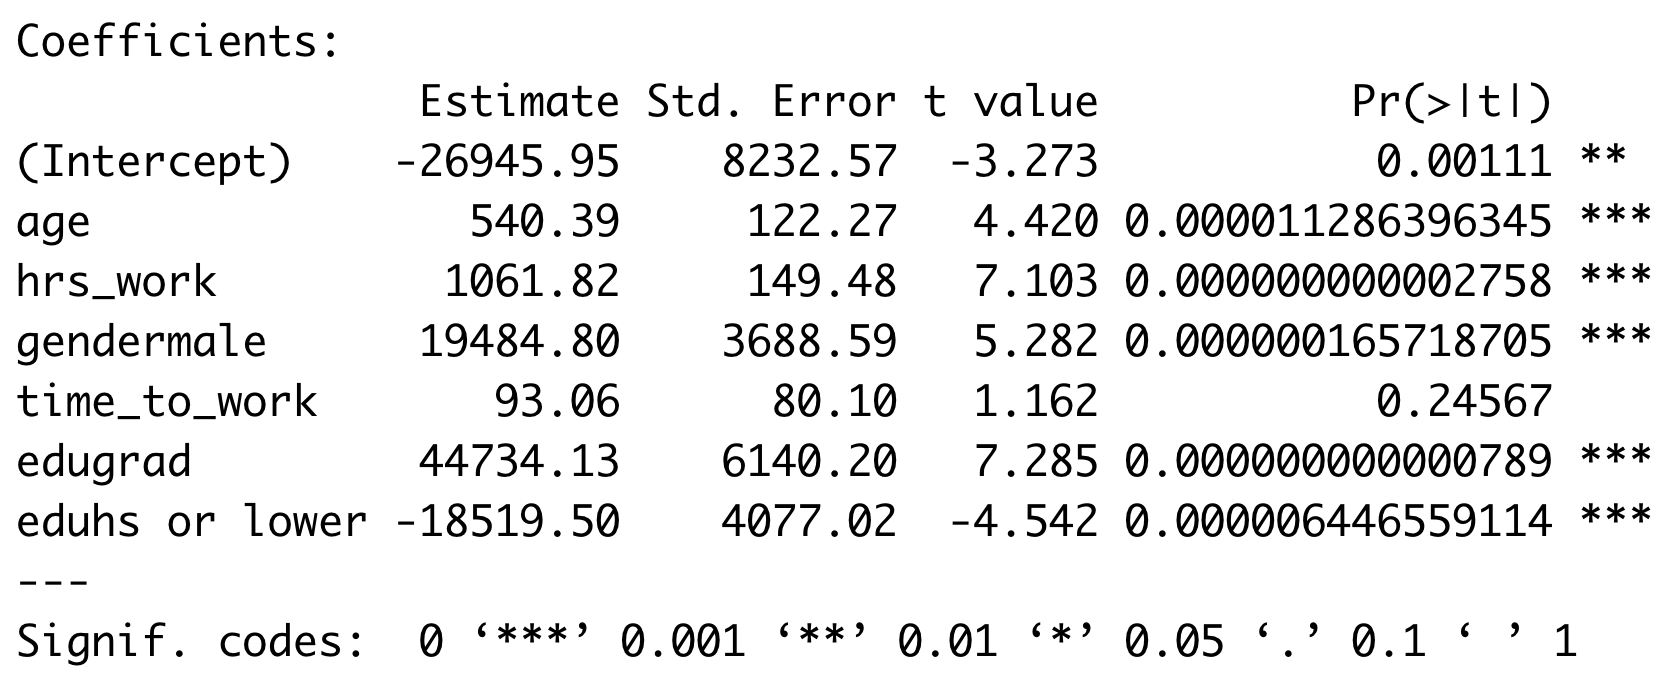
\includegraphics[scale=0.4]{income_v_age_full.png}
\end{center}

\end{frame}

%@@@@@@@@@@@@@@@@@@@@@@@@@@@@@@@@@@@@@@@@@@@@@@@@@
\begin{frame}
\frametitle{What does this actually look like? Gender and age...}
Example: the effect of gender on income depends on age:
\begin{center}
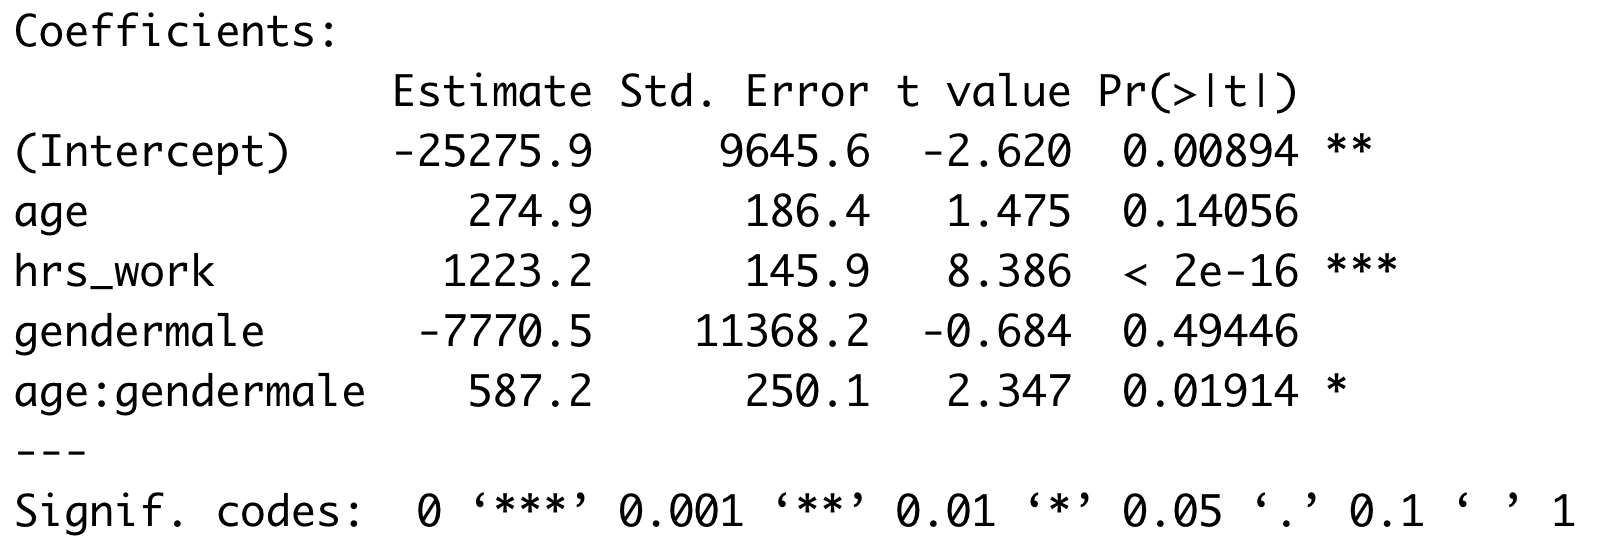
\includegraphics[scale=0.4]{age_gender_interaction.png}
\end{center}

\end{frame}

%@@@@@@@@@@@@@@@@@@@@@@@@@@@@@@@@@@@@@@@@@@@@@@@@@
\begin{frame}
\frametitle{Effect of gender on income is: $\beta_{\mbox{gender}} + \beta_{\mbox{age}}*\mbox{age}$}
\begin{center}
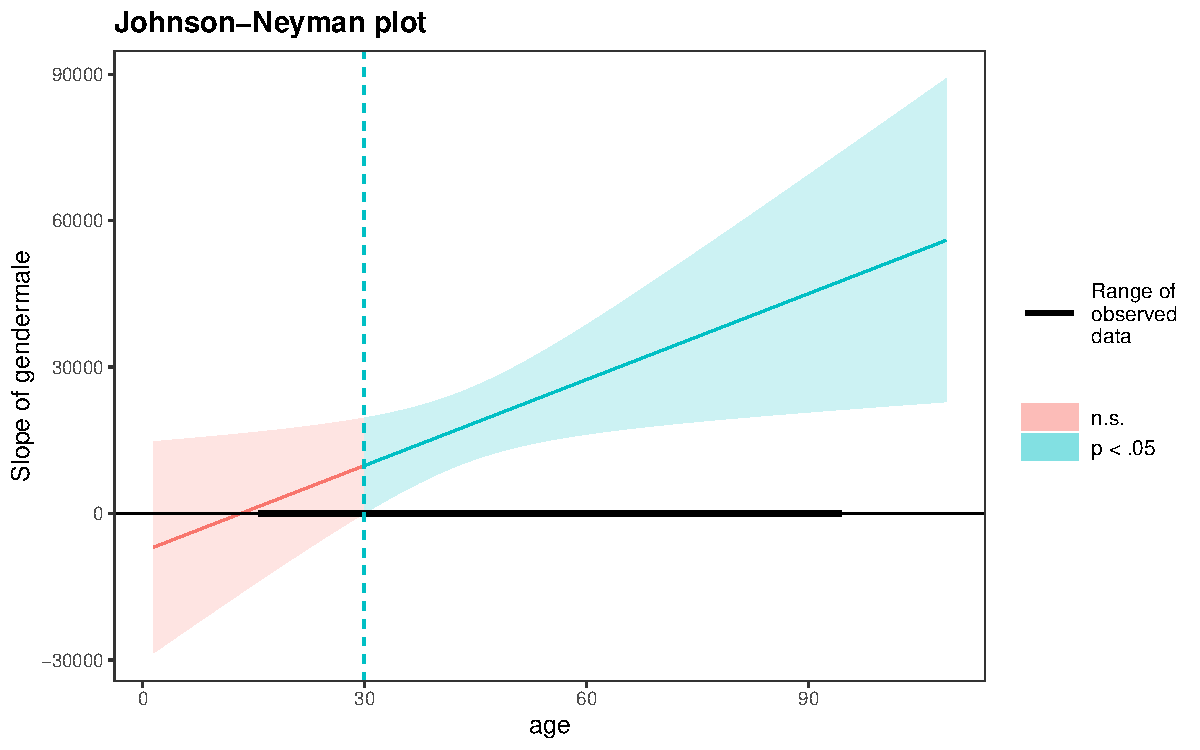
\includegraphics[scale=0.6]{age_gender.pdf}
\end{center}

\end{frame}

%@@@@@@@@@@@@@@@@@@@@@@@@@@@@@@@@@@@@@@@@@@@@@@@@@
\begin{frame}
\frametitle{What does this actually look like?  Age and hours worked...}
Example: the effect of age on income depends on hours worked:
\begin{center}
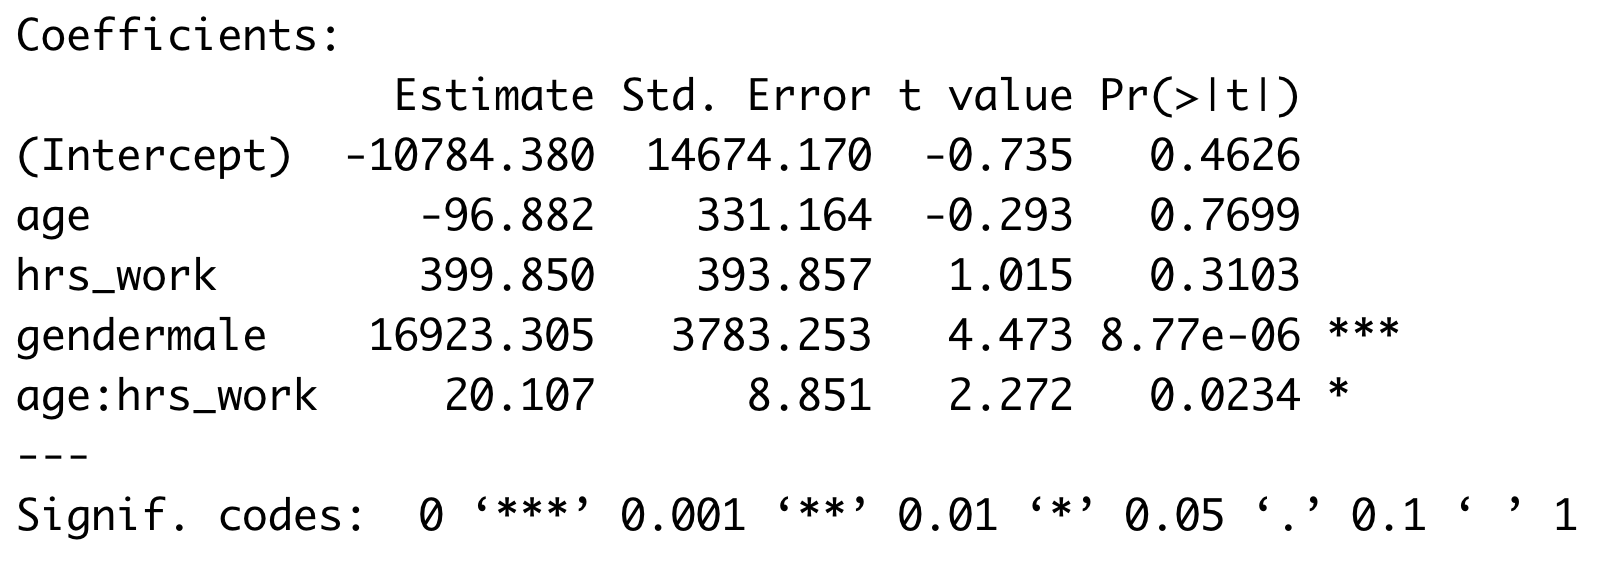
\includegraphics[scale=0.4]{age_hours_interaction.png}
\end{center}

\end{frame}

%@@@@@@@@@@@@@@@@@@@@@@@@@@@@@@@@@@@@@@@@@@@@@@@@@
\begin{frame}
\frametitle{Effect of age on income is: $\beta_{\mbox{age}} + \beta_{\mbox{hrs\_work}}*\mbox{hrs\_work}$}
\begin{center}
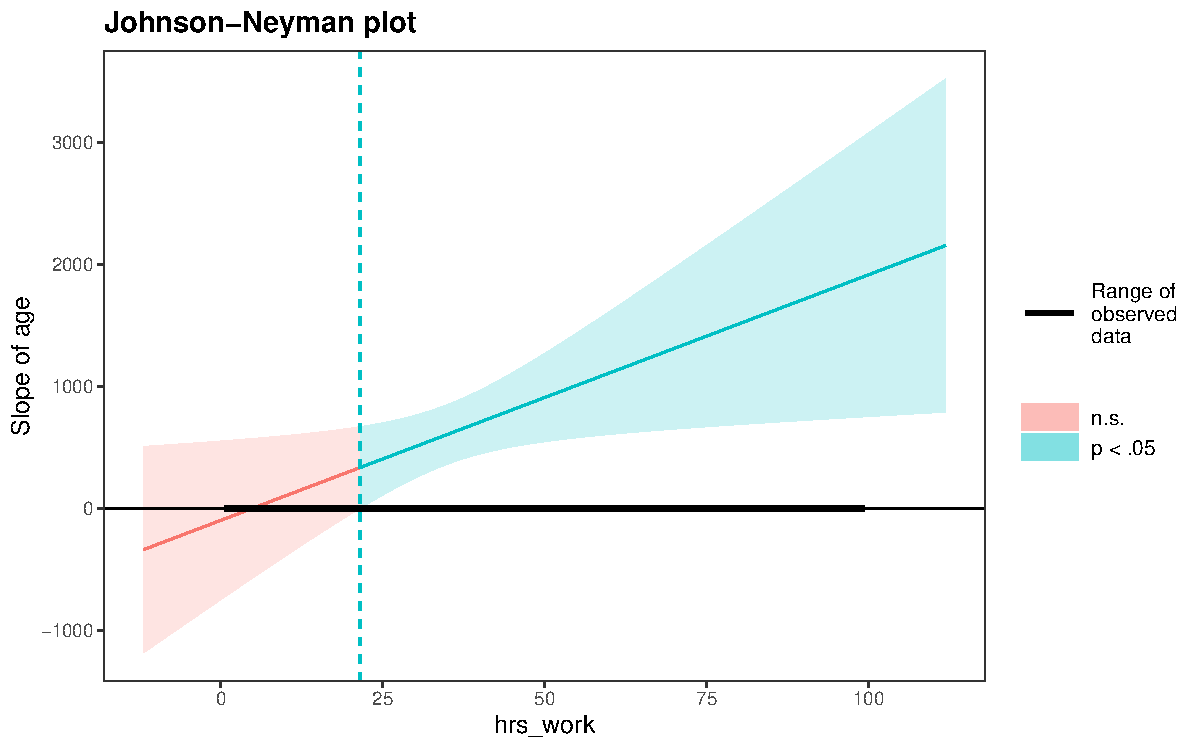
\includegraphics[scale=0.6]{age_hours.pdf}
\end{center}

\end{frame}

%@@@@@@@@@@@@@@@@@@@@@@@@@@@@@@@@@@@@@@@@@@@@@@@@@
\begin{frame}
\frametitle{Interpreting variable interactions: $p$-values}

\Large
\textbf{Fair warning} -- when you use interaction terms you can no longer just interpret $p$-values to determine whether to reject the null of no effect.

\end{frame}

%@@@@@@@@@@@@@@@@@@@@@@@@@@@@@@@@@@@@@@@@@@@@@@@@@
\begin{frame}

\begin{center}
\Huge\textbf{Why should we care?}\\
\bigskip
\bigskip
\large Linear regression can deal with complicated relationships between independent variables -- with careful design this can make it as powerful as modern machine learning techniques.\\
\end{center}

\end{frame}



\end{document}






